\documentclass[10pt, a4paper]{article}

\usepackage[a4paper, top=0.5cm, bottom=0.5cm, left=0.5cm, right=0.5cm, landscape]{geometry}
\usepackage{mathtools}
\usepackage{amsfonts}
\usepackage{multicol}
\usepackage{setspace}
\usepackage{graphicx}
\usepackage[dvipsnames]{xcolor}
\usepackage{array}



\author{Zachary Chua Yan Ern}
\date{February 2022}
\setstretch{1.25}

\newcommand{\highlight}[1]{{\color{red}\textbf{#1}}}
\newcommand{\blue}[1]{{\color{MidnightBlue}#1}}
\newcommand{\red}[1]{{\color{red}#1}}
\newcommand{\green}[1]{{\color{PineGreen}#1}}
\newcommand{\header}[1]{{\normalsize\textbf{#1}}}
\newcommand{\tab}[0]{\hspace*{2mm}}

\begin{document}
	\scriptsize %tiny
	\setlength\parindent{0pt}
	\setlength{\columnseprule}{0.1pt}
	
	\begin{center}
		{\large CS3243 CheatSheet}
	\end{center}
	
	\begin{multicols*}{3}
		\header{Agents and Environment}

		\textbf{Agent Components}

		% Sensors and Actuators

	  	- Sensors: information about the env

	  	\tab - Percept data at $t, p_{t}$, Percept History, $P = {p_{1}, ..., p_{t}}$

	  	- Actuators: how agent interacts with environment, set of \blue{Actions} $A$

	  	\green{Agent function $f: P \rightarrow a$}, where $a$ is a selected action given $P$

	  	Agent is \red{rational} if \red{optimises} performance measure (quantifiable objective), given percept seq, prior knowledge, set of actions, performance measure

	  	\highlight{Note:} do \textbf{not} assume agent is omniscient.

	  	% \textbf{Types of agents}

	  	% 1. Reflex Agents

	  	% \tab - uses \texttt{if-else} to make decisions, direct mapping of percepts to actions

	  	% \tab - domain specific, impractical for large search space

	  	% 2. Model-based reflex agent

	  	% \tab - makes decisions based on an internalised model

	  	% \tab - eg logical agents / bayesian networks

	  	% 3. Goal / Utility-based agents

	  	% \tab - Given \red{state, actions and goals / utility}

	  	% \tab - Determine \green{seq of actions} to reach goal / max utility

	  	% \tab - uninformed / informed search, Local Search, CSP, Adversarial Search

		% \textbf{AI as Graph Search}

	  	% - Each percept corresponds to a state in the problem (state $\rightarrow$ vertex)

	  	% - Define desired (goal) states

	  	% - After action, arrive at new state (actions are edges)

	  	% - Search space is graph

		\textbf{Problem Env}

	  	\begin{tabular}{ | m{1.5cm} | m{1.5cm} | m{5cm} | }
		\hline
		Fully observable & Partially observable & Whether can sense all information\\
		\hline
		Deterministic & Stochastic & can determine next state from $a$, $s$? \\
		\hline
		Episodic & Sequential & episodic: action impacts current state, sequential: actions impact future states\\
		\hline
		Discrete & Continuous & for state information\\
		\hline
		Single & Multi agent & other entities that influence agent behaviour, competing or cooperating\\
		\hline
		Known & Unknown & Knowledge of agent (goal state)\\
		\hline
		Static & Dynamic & env change while deciding action?\\
		\hline
	  	\end{tabular}

	  	\header{Path Planning}

	  	\textbf{Properties}

	  	Environment --- Fully observable, Deterministic, Discrete, Episodic (plan solution, plan is formed sequentially)

		\textbf{Problem Formulation}

		State: representation of instance of environment

		Node: Element in frontier representing current path traversed

		\tab - State, Parent Node, Action, Path Cost, Depth

		Goal Test function, Actions function, Action costs function ($\geq 0$)

		Transition Model function: takes in a state, applies action, returns new state

		\textbf{Algo Criteria}

		Efficiency - space and time

		\green{Complete} - find a solution if exists, correctly report failure it does not

		\green{Optimal} - solution with \blue{lowest} path cost among all solutions

		\textbf{Types of search}

		Tree Search
		
		\tab - Can revisit states, allows redundant paths, including cycles

		\tab - Incomplete, if there are cycles

		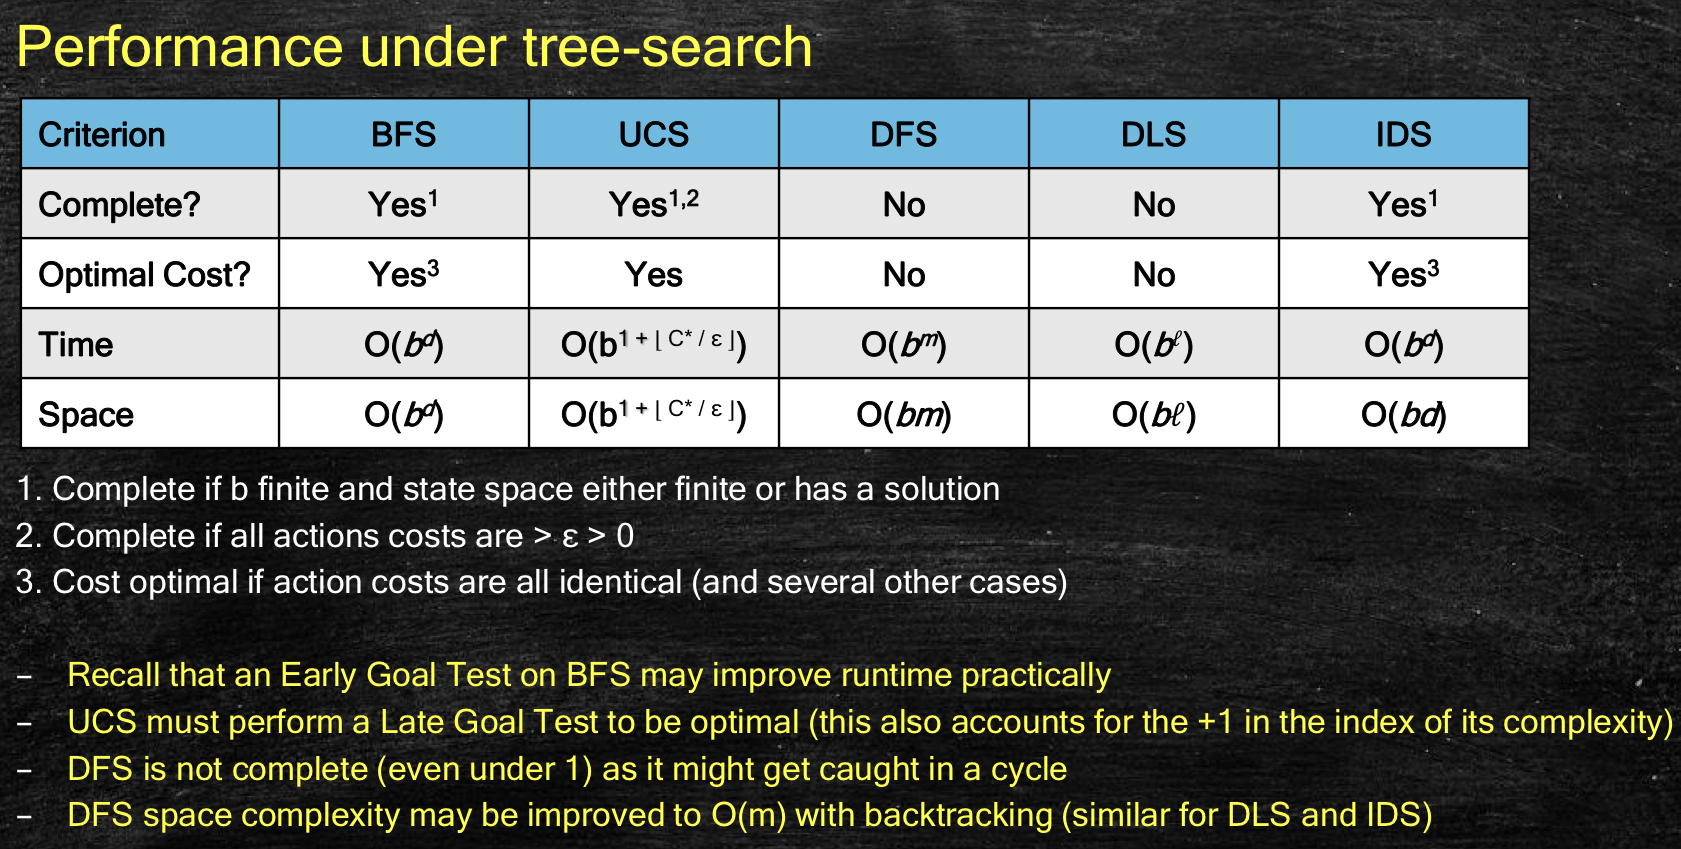
\includegraphics[scale=0.15]{./assets/treeSearch.png}

		Graph Search

		\tab - Add nodes to \texttt{reached} hash table on pop 

		\tab - Only add new node to frontier (and \texttt{reached}) if

		\tab \tab 1. state represented has not been reached before

		\tab \tab 2. path to state already reached is cheaper than the stored one

		\highlight{NOTE:} Do \red{not} need to allow cheaper paths for BFS DFS as costs doesnt matter and not optimal

		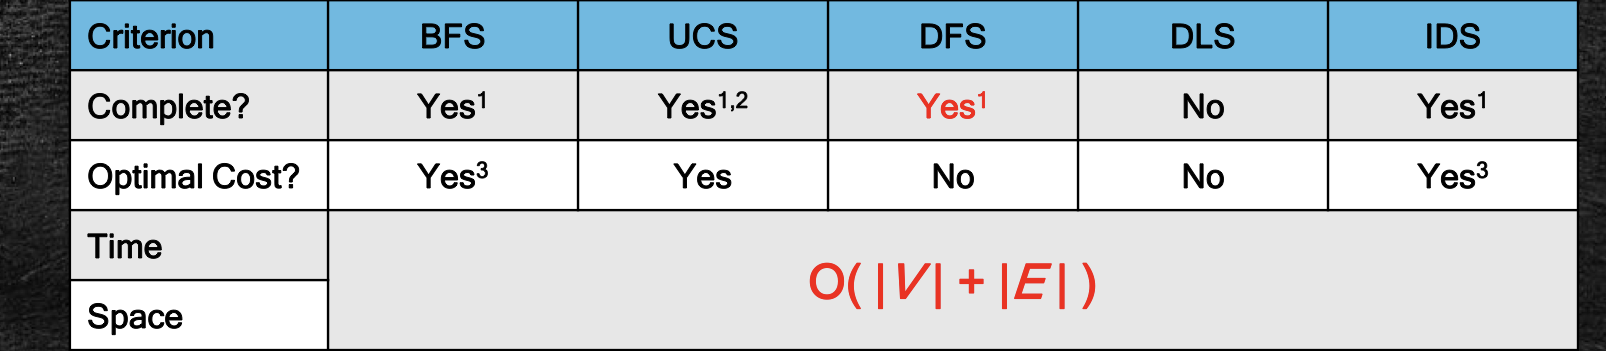
\includegraphics[scale=.15]{./assets/graphSearch.png}

		Limited Graph Search V1: Adds to \texttt{reached} \red{on push}

		\tab{} - \red{Not optimal} for UCS or A*

		Limited Graph Search V2

		\tab - Adds to \texttt{reached} on \red{pop}, \red{does not} check if path is cheaper 

		\tab - \green{Optimal} for UCS or A* (w consistent heuristic)\\

		\header{Uninformed Search}

		\textbf{BFS - Queue}

		% Time: $O(b^{d})$, Space: $O(b^{d})$, $b$: branching factor, $d$: depth of shallowest goal

		% \green{Complete} if finite space / solution, \red{not optimal} unless costs uniform

		\green{Optimised} with \red{early goal test} (goal test on push to frontier instead of pop)

		\textbf{UCS aka Dijkstra - PQ, path cost}

		% Time: $O(b^{e})$, Space: $O(b^{e})$

		% $e$: $1 + \lfloor \frac{C*}{\epsilon} \rfloor$, where C* is the optimal path cost

		% $\epsilon$: small positive constant, smallest action cost

		\green{Complete} if finite space / solution, \green{Optimal} with tree, graph and limited V2

		\textbf{DFS - Stack}

		% Time: $O(b^{m})$, Space: $O(bm)$, $m$: max depth

		% \red{Not complete} unless finite search space, \red{not optimal}

		\red{Note}: space $O(m)$ with backtracking (assume fixed order of actions)

		\textbf{Depth Limited Search (DLS)}

		DFS with depth limit $l$

		% Time: $O(b^{l})$, Space: $O(bl)$

		% \red{Not complete, Not Optimal}

		\textbf{Iterative Deepening Search (IDS)}

		Use DLS recursively, each time increasing $l$ by 1

		\tab - Completeness of BFS with space complexity of DFS

		Overhead: rerun top levels many times ($\sim11\%$)

		\tab - Nodes generated by DLS: $O(b^{0} + b^{1} + ... + b^{l})$

		\tab - Nodes generated by IDS: $O((d + 1)b^{0} + db^{1} + ... + b^{d})$\\

		% Time: $O(b^{d})$, Space: $O(bd)$

		% Complete / Optimal: same as BFS

		\header{Informed Search}

		Use domain knowledge to estimate cost from $s$ to $G$, heuristic function $h$

		Define \red{evaluation function} $f$ to be used as priority function in PQ

		UCS: $f = g$

		% 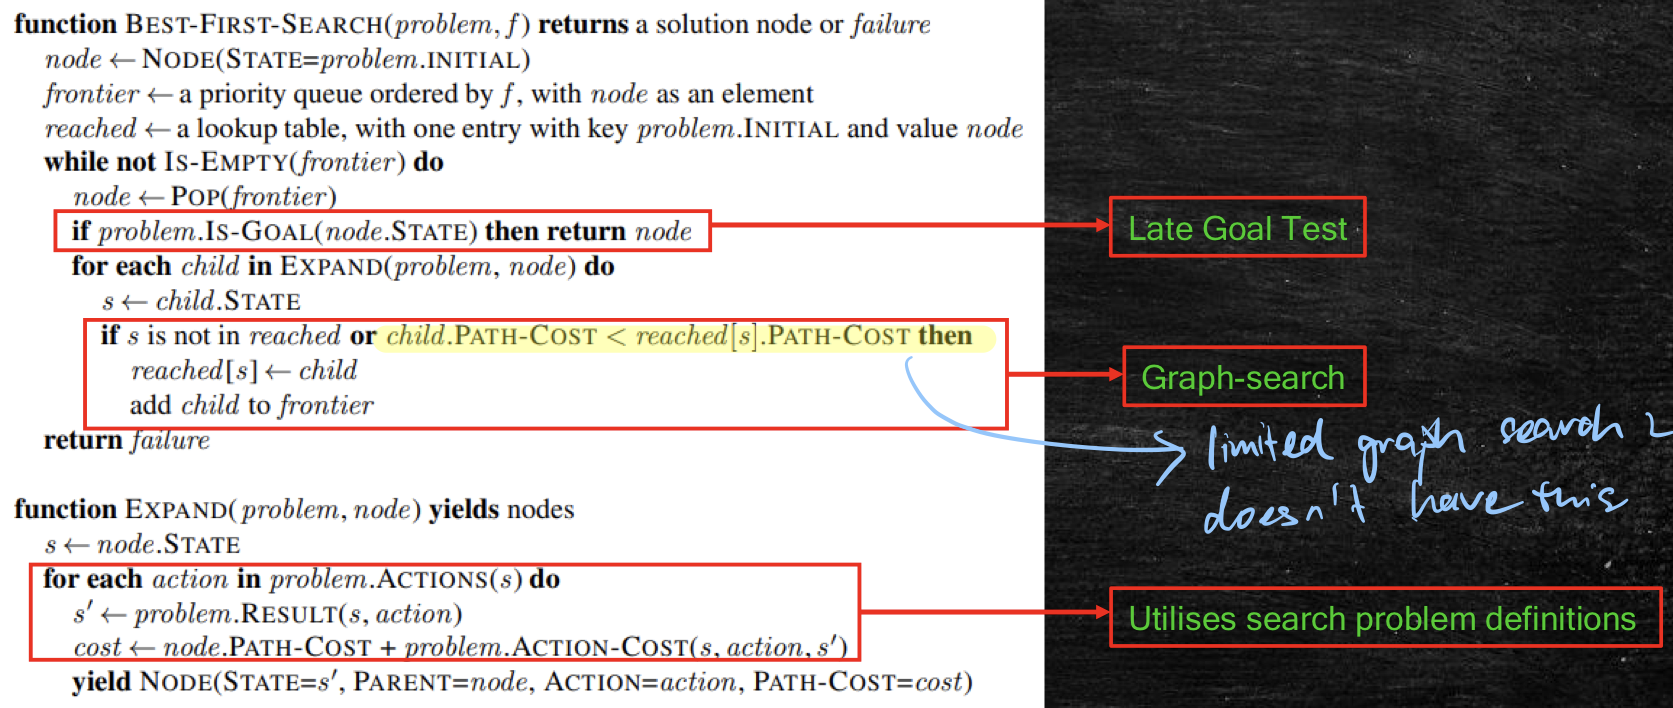
\includegraphics[scale=.16]{./assets/bestFirst.png}

		\textbf{Greedy Best First Search}

		Evaluation fn: \green{$f(n) = h(n)$}

		\red{Not optimal} does not take into consideration cost of path travelled

		Tree Search: \red{Not complete}, stuck between 2 nodes with lowest $h$ values

		Graph Search: \green{Complete}, if search space is finite

		\textbf{A* Search}

		Evaluation fn: \green{$f(n) = g(n) + h(n)$}

		Optimality:

		\tab Admissible heuristic: Tree Search, Graph Search

		\tab Consistent heursitic: Tree, Graph, Limited Graph V2

		A* and Graph Search \red{costly} due to updates (need update descendants)\\

		\header{Heuristics}

		\textbf{Admissible}, underestimate cost, 0 at goal

		$\forall n, h(n) \leq h^{*}(n)$

		\textbf{Consistent}, $f$ monotonically $\uparrow$ along path, admissible if value at goal = 0

		$\forall n, n', h(n) \leq cost(n, a, n') + h(n')$

		\textbf{Dominance}

		if $\forall n, h_{1}(n) \geq h_{2}(n)$, then $h_{1}$ dominates $h_{2}$

		- if $h_{1}$ is also admissible: $h_{1}$ \green{closer} to $h^{*}$, $h_{1}$ more \green{efficient} than $h_{2}$

		\highlight{Note}: for 3243, $h_{1}$ and $h_{2}$ need not be admissible

		\textbf{Creating heuristics}

		- Want \green{efficient} $h$, close to $O(1)$

		- Want \green{admissible}, consistent harder

		\textbf{Relaxing constraints}: gives admissible heuristics, $\uparrow$ relaxed, $\downarrow$ dominant

		\textbf{Top Down Approach}

		- What dep var to model / approx, and indep vars help to calculate these?

		\textbf{Bottom up Approach}

		- What vars can be efficiently calculated, and what can these variables model?\\

		\header{Local Search}: Have goal test, want goal state values, no need path

		- Greedy \red{not} systematic

		- Space Complexity: $O(b)$, only store node and successors

		\textbf{State formulation}

		- no partially filled states, each state is a potential solution

		- ``guess'' a solution, ``check'' its value

		- ``systematic guess'': move to states of higher value (closer to goal)

		\textbf{Steepest Ascent Hill Climbing Algorithm}

		% 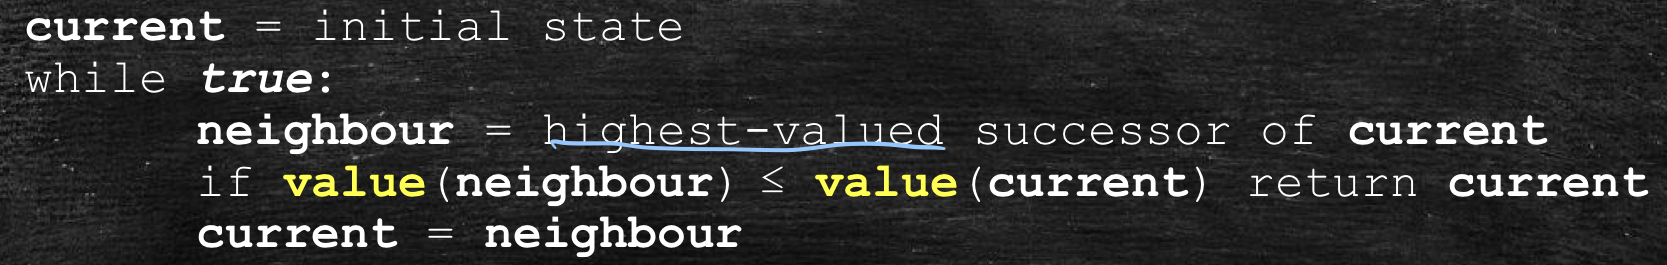
\includegraphics[scale=0.15]{./assets/steepestAscent.jpeg}

		- Only store current state

		- On each iteration, find successor that \textbf{improves} on current state

		\tab - Requires \red{\texttt{actions}} and \red{\texttt{transitions}} to determine successor

		\tab - Requires \red{\texttt{value}}: a way to assign each state a value ($f(n) = -h(n)$)

		- If none exists, return current state as the best option

		- \highlight{Can fail}, return non-goal, fail at \red{local maxima, shoulder \ plateau, ridge}

		\textbf{Variants}

		- Sideways move: replace $\leq$ with $<$, \green{Can traverse shoulder}

		- Stochastic: chooses randomly among states with values better than current

		\tab -\green{ try to prevent getting stuck at local maxima }

		- First Choice: randomly generate successors, choose first one that is better

		\tab - \green{Similar to stochastic, handles high $b$}

		- Random restart: outer loop to randomly pick new start until solution found

		\tab - \green{Guaranteed to find solution}

		\textbf{Analysis}

		$p_{1}$ be $P(success)$, $n_{1}, n_2$ be no. of steps of expected success, of expected failure

		\centerline{Expected Computation = $n_{1} + \frac{1 - p_{1}}{p_{1}} * n_{2}$}

		\textbf{Local Beam Search}

		1. Begin with $k$ random starts

		2. Each iteration generate successors for \red{all} $k$ states

		3. Repeat with best $k$ among \red{all} successors unless goal found

		Better than k // RR, best $k$ from \highlight{all} successors, not from successors, $k$ times

		\textbf{Stochastic Beam Search}: Similar to stochastic hill climbing\\

		\header{Constraint Satisfaction Problem}

		\textbf{State Representation:}

		- Variables: $X = {x_{1}, x_{2}, ... , x_{n}}$, Domains: $D = {d_{1}, d_{2}, ... , d_{n}}$

		\tab - such that $x_{i}$ has domain $d_{i}$

		- Initial State: all unassigned, Intermediate State: partial assignment

		\textbf{Goal Test}

		- Constraints: $C = {c_{1}, c_{2}, ... , c_{m}}$

		- Each $c_{i}$ describes necessary relationship $rel$, between set of variables $scope$

		\tab - eg. $scope = (x_{1}, x_{2})$ and $rel = x_{1} > x_{2}$

		- constraints can be \red{unary, binary, global}

		Actions, Transitions - costs, evaluation function not utilised

		\textbf{Objective:} find \green{complete} (all variables assigned) and \green{consistent} (all constrainst satisfied) assignment

		\textbf{CSP search algo}

		% 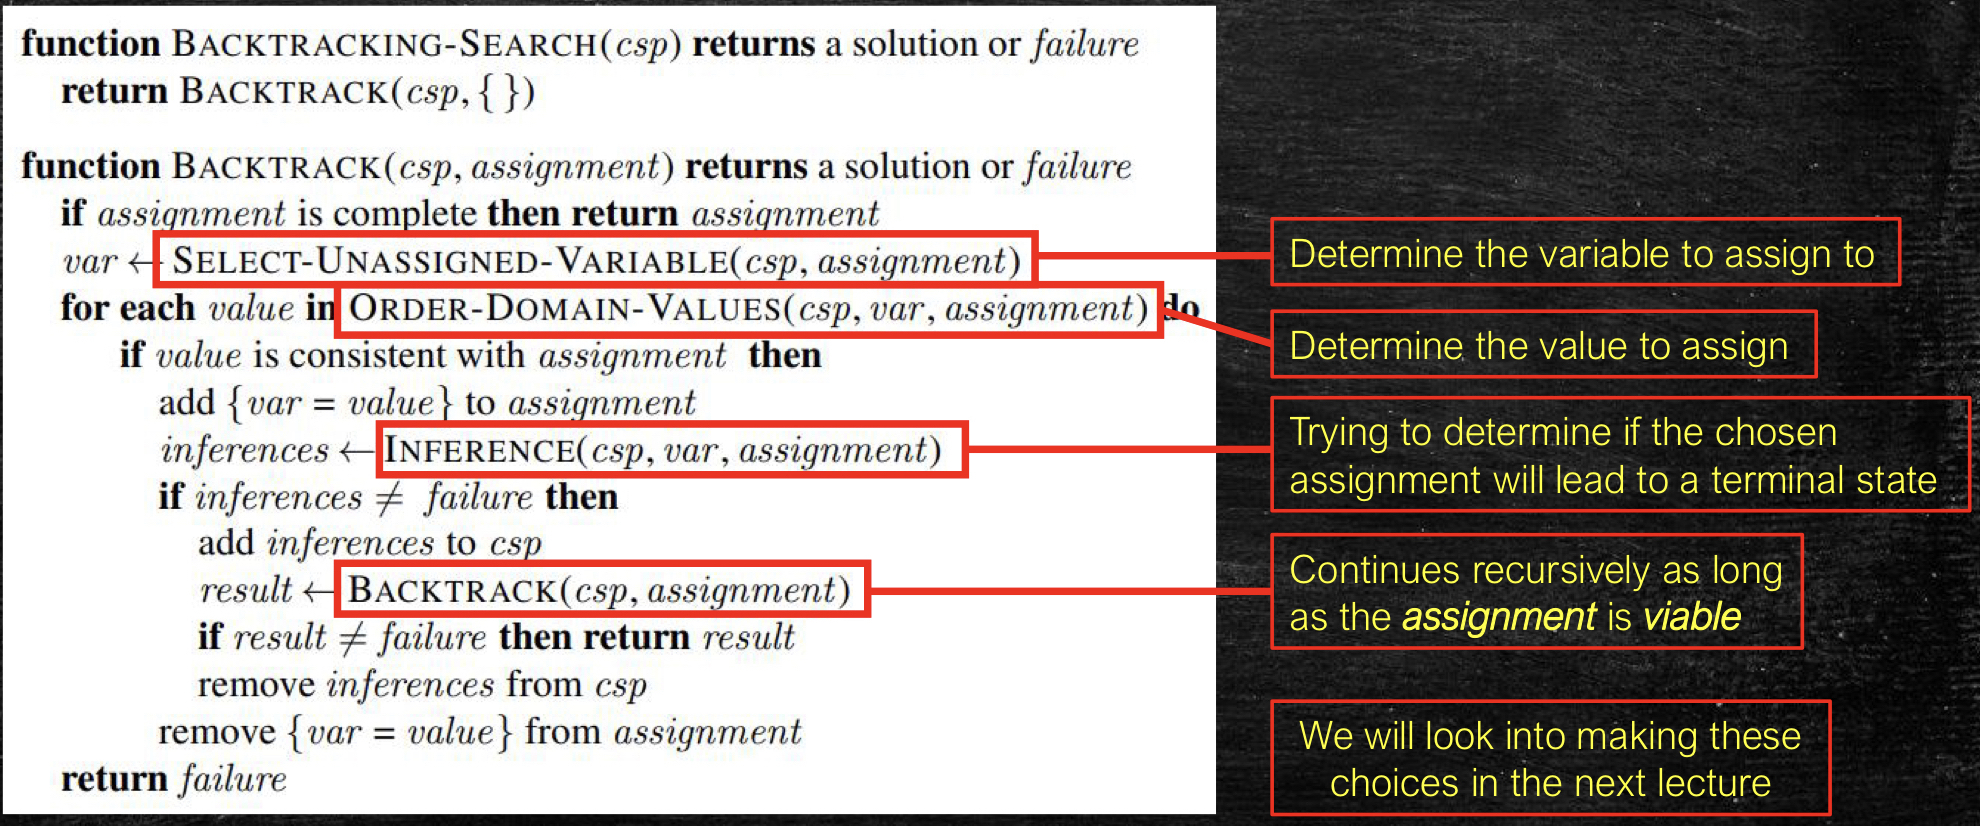
\includegraphics[scale=0.135]{./assets/CspBacktracking.jpeg}

		- Use DFS as solutions \green{are all at} max depth

		- Each level assign to \green{1 variable}, as order does not matter (prunes tree)

		- Backtrack when there are no legal assignments

		\textbf{Variable Order Heuristics} --- fail first (have to assign to all variables)

		1. Min Remaining Values Heuristic - choose var with least legal values

		\tab{} Places \red{larger} subtrees closer to root, prunes them earlier

		2. Degree Heuristic - var that restricts most no. of other vars (reduces $b$)

		\tab{} Break MRV ties with Degree, MRV $\rightarrow$ Degree $\rightarrow$ random

		\textbf{Value Order Heuristics} --- fail last, only need to assign one value 

		1. Least Constraining Value - value that rules out fewest choices

		\tab{} Avoids failure, leaving maximum flexibility for subsequent assignments

		\textbf{Inference} --- Detect if heading for failure early

		1. Forward Checking --- track reminaing legal values for unassigned vars

		\tab{} After assign, remove constraint violating values from neighbours' domain

		\tab{} Terminate search when no legal values left

		\tab{} \red{Problem}: does \red{not} provide early detection for all failures

		2. Constraint Propagation --- remove values inconsistent w constraints

		\tab{} \green{Node-consistent} (unary) and \blue{Arc-consistent} (binary)

		2.1 Node --- done as pre-processing, remove values violating unary constraint

		2.2 Arc Consistency --- domain is consistent with related binary constraints

		\textbf{Definition:} $X_i$ is arc-consistent wrt $X_j$ (arc($X_i$, $X_j$) is consistent) \highlight{iff} 
		$\forall x \in D_i$, $\exists y \in D_j$ that satisfies binary constrain on arc($X_i$, $X_j$)

		\tab{} - Domain values \green{must have partnering domain value} in other variable

		\highlight{Note}: If $X_i$ is updated, arcs w $X_i$ as target \red{must be rechecked}, the arc causing the update

		Values removed from $X_i$ have no values in $X_j$ satisfying constraint, so there must not be any value in $X_j$ requiring that value in $X_i$ either

		\highlight{Note}: Each binary constraint becomes 2 arcs, 1 for each direction

		\includegraphics*[scale=.14]{./assets/AC3.jpeg}

		\textbf{Time Complexity $O(n^2d^3)$} --- at most $2 \times nC2$ arcs ($O(n^2)$), each arc can be inserted $d$ times, checking consistency is $O(d^2)$

		\textbf{Usage} --- Preprocessing / After variable assignment 
		
		After assignment: Inference to update domain, check for terminal state, only initialise queue w arcs of \red{neighbouring unassigned variables}, wrt current node\\
		
		\header{Adversarial Search}

		\red{2} players,  \red{0 sum} game, \green{deterministic}, \green{turn-taking}

		\textbf{State Representation and functions} --- representation depends on game

		- \texttt{to\_move(s)}: player's turn, \texttt{actions(s)}: legal actions
		
		- \texttt{result(s, a)}: transition model, returns resultant state 
		
		- \texttt{is\_terminal(s)}: \texttt{true} when game over, \texttt{false} ow, 
		
		- \texttt{utility(s, p)}: p's \red{numeric} value in \red{terminal} state (1 win, 0 draw, -1 lose)

		\textbf{Strategies}: specifies behaviour for every node in the game

		Winning Strategy: for any strategy by Player 2, Player 1 wins

		Non-losing Strategy: for any strategy by Player 2, Player 1 wins or draws

		\textbf{Minimax} - DFS Traversal of game tree w backward induction on utility

		% \tab{} - \texttt{utility} if terminal state, \green{max} if \green{max} player, \red{min} if \red{min} player

		\green{Complete} (if game tree finite), \green{Optimal}, Time: $O(b^m)$, Space: $O(bm)$

		\textbf{$\alpha$-$\beta$ pruning} - Don't explore moves that will never be considered

		- \red{Lower} bound $\alpha$ on \green{MAX's} values, \green{Upper} bound $\beta$ on \red{MIN's} values

		\textbf{Pruning Rules:}

		1. \red{Min} node $n$, stop searching below $n$ if MAX ancestor i, \highlight{$\alpha (i) \geq \beta (n)$}

		2. \green{Max} node $n$, stop searching below $n$ if MIN ancestor i, \highlight{$\beta (i) \leq \alpha (n)$}

		\textbf{Analysis}- Perfect ordering $O(b^{m / 2})$, random $O(b^{3m/4})$ for b $<$ 1000

		\highlight{Problem} - depth of tree large

		\green{Solution} - Heuristic Minimax (cutoff depth $\rightarrow$ evaluation function)

		\red{Note}: evaluation fn at non-terminal nodes, utility fn at terminal nodes

		\textbf{Stochastic Games}: calculate expected value of a state\\

		\header{Knowledge Representation} --- logical agents

		\textbf{Logical Agents}: Represent agent \green{domain knowledge} using \green{logical formulas}

		- Used to make inferences on existing info

		- Inference Engine: \green{Domain-independent} algos

		- Knowledge Base: \red{Domain-specific} content

		\textbf{Knowledge Base (KB)}: Formal language, pre-populated with rules

		% \textbf{KB Agent function}

		% \includegraphics*[scale=0.135]{./assets/KBAgent.jpeg}

		\textbf{Modelling}
		$v$ \red{models} $\alpha$ if $\alpha$ is \green{true} under $v$, $v$ is a value assingment 

		$M(\alpha)$ is the set of all models for $\alpha$

		\textbf{Entailment}: one thing follows from another, $\alpha \models \beta \equiv M(\alpha) \subseteq M(\beta)$ 

		\textbf{Inference Algorithm Properties}

		$KB \vdash _A \alpha$: $\alpha$ is inferred from $KB$ by inference algo $A$

		Soundness: $A$ is \green{sound} if $KB \vdash _A \alpha \rightarrow KB \models \alpha$

		Completeness: $A$ is \green{complete} if $KB \models \alpha \rightarrow KB \vdash _A \alpha$

		\textbf{Inference Algo - Truth Table Enumeration}

		\includegraphics*[scale=0.15]{./assets/TruthTable.jpeg}

		- Checks: ALL rows where $KB$ true, $\alpha$ true, ie. $M(KB) \subseteq M(\alpha)$

		- Depth first Enumeration

		- Time: $O(2^n)$, Space: $O(n)$

		- \green{Sound}: implements definition of entailment directly

		- \green{Complete}: Finite models to check

		\textbf{Validity and Satisfiability}
		
		$\alpha$ is \green{valid} if true for \highlight{ALL} truth assignments (tautologies)

		\tab{} - Deduction Theorem: $(KB \models \alpha) \leftrightarrow (KB \rightarrow \alpha)$ is valid

		Sentence is \green{satisfiable} if True for \highlight{SOME} truth assignment

		Sentence is \red{unsatisfiable} if True for \highlight{NO} truth assignment (contradictions)

		\tab{} - $(KB \rightarrow \alpha) \leftrightarrow (KB \wedge \neg \alpha)$ is unsatisfiable (proof by contradiction)

		\textbf{CNF}: Conjunction of Disjunctive sentences

		\textbf{Resolution}: proof by contradiction, tries to show $KB \wedge \neg \alpha$ is \red{unsatisfiable}

		$(P \vee x) \wedge (Q \vee \neg x)$ resolves to $P \vee Q$

		\includegraphics*[scale=0.14]{./assets/resolution.jpeg}

		1. if empty clause, can infer $\alpha$

		2. if no more resolutions and not empty clause, then cannot infer $\alpha$

		- empty clause is \red{disjunction of no literals}. Disjunction is true if at least one literal is true,
		so whole KB is false, $\neg \alpha$ is unsatisfiable

		- \green{Sound}: Inference rules used to generate new clauses are sound, monotonicity

		- \green{Complete}: resolution closure (not covered)\\

		\header{Uncertainty and Bayesian Networks}

		\textbf{Joint Probability}: $(x, y) \in D_X \times D_Y = p_{X, Y}(x, y) = P(X = x, Y = y)$

		$p_X(x) = \sum_{y \in D_Y} p_{X, Y}(x, y)$

		\textbf{Bayes Rule}: $P(A | B) = \frac{P(B | A)P(A)}{P(B)}$

		\textbf{Chain Rule}: $P(R1, \dots, R_k) = \prod_{j = 1, \dots, k} P(R_j | R_1, \dots R_{j - 1})$

		\textbf{Inference via Baye's Rule}: $P(\alpha | R_1, \dots , R_k)$

		\textbf{Size of join distribution table}

		$n$ RVs, each with domain size $d$ $\rightarrow d^n - 1$ (last entry can be inferred)

		$n$ indep RVs, each with domain size $d \rightarrow dn$

		\textbf{Chain Rule with Conditional Independence}

		$P(T_1, \dots, T_k, S)  = P(T_1|S) \dots P(T_k|S) P(S)$

		join distribution size = $n + 1$ (linear), cond indep more robust than indep

		\textbf{Conditional Indep, Bayes, Normalisation}

		Given causes that result in indep effects,

		$P(C | E_1, \dots, E_k) = \alpha P(C) P(E_1 | C) \dots P(E_k|C)$

		where $\alpha = \frac{1}{P(E_1,\dots , E_k)}$
		
		Conditional Probability Table only needs $k + 1$ entries ($k$ effects)

		- Each $P(E_i | C)$ and $P(C)$

		\textbf{Bayesian Networks}

		Represents join distributions as a graph, \red{vertices} are r.v, \red{edge} $X \rightarrow Y$ indicates X causes Y

		\red{Conditional Distribution} for each node given its parents $P(X | Parents(X))$, ie. Probability distribution for X given \red{each combination of Parents}

		EG.

		1. $A \rightarrow C, B \rightarrow C = P(C|A,B) P(A)P(B)$

		2. $A \rightarrow B, A \rightarrow C = P(C|A)P(B|A)P(A)$ \highlight{note $P(A)$ not $P(A)^2$}

		3. $A \rightarrow B, B \rightarrow C = P(C|B)P(B|A)P(A)$

		\textbf{Size of Join Distribution in Bayesian Networks}

		Rows in CPT for Boolean $X$ with $k$ parents $ = 2^k$, each row require one $p$ for when X = true

		If each $X_i$ has $\leq k$ parents, then need $O(n2^k)$ values

		\textbf{Constructing BN}

		1. Choose an ordering of $X_1, \dots, X_n$ (ordering impt but not in 3243)

		2. For $i = 1, \dots , n$

		2.1 Add node $X_i$ into network 

		2.2 Select Minimal set of parents from $X_1, \dots, X_{i - 1}$, such that 

		\centerline{$P(X_i | Parents(X_i)) = P(X_i|X_1, \dots , X_{i - 1})$}

		\red{Note}: Check all subsets ($O(2^{i - 1})$), determines which nodes influence $X_i$

		2.3 Link every parent to $X_i$

		2.4 Write down \red{CPT} for $P(X_i | Parents(X_i))$







		






		
		




	\end{multicols*}
\end{document}
